\documentclass[11pt]{article}
\usepackage[utf8]{inputenc}
\usepackage{amsmath,amssymb}
\usepackage{geometry}
\usepackage{tikz}
\usepackage{booktabs}
\usepackage{caption}
\geometry{a4paper,margin=1in}
\setcounter{secnumdepth}{0}

% Plot styles shared by all figures (pure TikZ).
\tikzset{
  fn/.style={thick, smooth, samples=161},
  dfn/.style={thick, dashed, smooth, samples=161},
  ref/.style={thin, gray!60, smooth, samples=161},
  guide/.style={very thin, gray!50, dotted},
}
% \axes{xmin}{xmax}{ymin}{ymax}
\newcommand{\axes}[4]{%
  \draw[->] (#1,0) -- (#2,0) node[right] {$z$};
  \draw[->] (0,#3) -- (0,#4);
  \foreach \t in {-4,-2,2,4} \draw (\t,0.04) -- (\t,-0.04) node[below] {\scriptsize $\t$};
}

\title{Activation Functions: Sigmoid, tanh, arctan, ReLU and Softmax}
\author{Haiyi Li}
\date{}

\begin{document}
\maketitle

\section{Why we need them}

A neuron computes a pre-activation and then applies an activation function $\phi$:
\begin{equation}
  z = w^\top x + b, \qquad a = \phi(z).
\end{equation}
Without $\phi$, stacking layers gives nothing new:
\begin{equation}
  W_2(W_1x+b_1)+b_2 = (W_2W_1)\,x + (W_2b_1+b_2),
\end{equation}
which is still one linear map. So depth only helps when $\phi$ is nonlinear.

For training, $\phi'$ matters as much as $\phi$. Take a chain with one unit per layer,
$a_l=\phi(z_l)$ and $z_{l+1}=w_{l+1}a_l$. By the chain rule
\begin{equation}
  \frac{\partial a_L}{\partial z_1}
  = \phi'(z_L)\prod_{l=1}^{L-1} w_{l+1}\,\phi'(z_l).
  \label{eq:chain}
\end{equation}
If $|\phi'|$ is small, this product shrinks with $L$ (vanishing gradient).
Below, each function is described by its formula, range, derivative,
and how fast $\phi'$ decays for large $|z|$.

\section{Sigmoid}

\begin{equation}
  \sigma(z)=\frac{1}{1+e^{-z}}, \qquad \sigma(z)\in(0,1), \qquad \sigma(0)=\tfrac12 .
\end{equation}
It is symmetric about the point $(0,\tfrac12)$:
\begin{equation}
  \sigma(-z)=1-\sigma(z).
\end{equation}
The derivative can be written with $\sigma$ itself:
\begin{equation}
  \sigma'(z)=\frac{e^{-z}}{(1+e^{-z})^2}=\sigma(z)\bigl(1-\sigma(z)\bigr),
  \qquad \max_z \sigma'(z)=\sigma'(0)=\tfrac14 .
  \label{eq:sigmoid-derivative}
\end{equation}
For large $|z|$,
\begin{equation}
  1-\sigma(z)=\frac{1}{1+e^{z}}\approx e^{-z}\ (z\to+\infty),
  \qquad \sigma'(z)\approx e^{-|z|}.
\end{equation}

Two problems follow.
First, with $\sigma'\le\tfrac14$, \eqref{eq:chain} gives
\begin{equation}
  \left|\frac{\partial a_L}{\partial z_1}\right|
  \le \left(\tfrac14\right)^{L}\prod_{l=1}^{L-1}|w_{l+1}|,
  \qquad \left(\tfrac14\right)^{10}\approx 9.5\times10^{-7}.
\end{equation}
Second, $\sigma(z)>0$ always. For a unit with inputs $a_j=\sigma(z_j)$ and error signal $\delta$,
\begin{equation}
  \frac{\partial \ell}{\partial w_j}=\delta\,a_j ,
\end{equation}
so all $\partial\ell/\partial w_j$ share the sign of $\delta$ and the weights move in a zig-zag.

\begin{figure}[h]
\centering
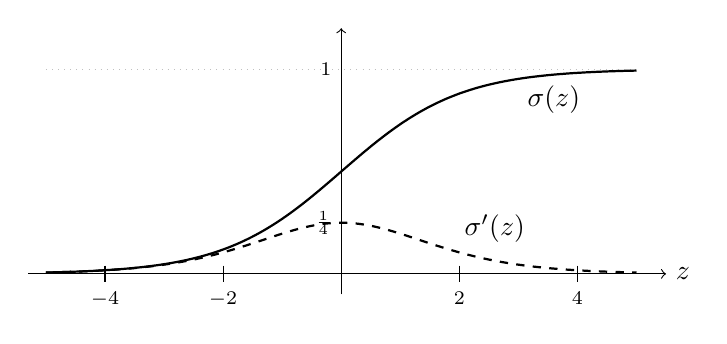
\begin{tikzpicture}[x=0.75cm,y=2.6cm]
  \axes{-5.3}{5.5}{-0.1}{1.2}
  \draw[guide] (-5,1) -- (5,1);
  \node[left] at (0,1) {\scriptsize $1$};
  \draw[fn, domain=-5:5] plot (\x, {1/(1+exp(-\x))});
  \draw[dfn, domain=-5:5] plot (\x, {(1/(1+exp(-\x)))*(1-1/(1+exp(-\x)))});
  \node[left] at (0,0.25) {\scriptsize $\tfrac14$};
  \node at (3.6,0.85) {$\sigma(z)$};
  \node at (2.6,0.22) {$\sigma'(z)$};
\end{tikzpicture}
\caption{Sigmoid (solid) and its derivative (dashed). The derivative never exceeds $1/4$.}
\end{figure}

\section{Hyperbolic tangent}

\begin{equation}
  \tanh z=\frac{e^{z}-e^{-z}}{e^{z}+e^{-z}}, \qquad \tanh z\in(-1,1), \qquad \tanh 0=0 .
\end{equation}
It is a rescaled sigmoid:
\begin{equation}
  \tanh z = 2\sigma(2z)-1,
  \qquad\text{since}\quad
  2\sigma(2z)-1=\frac{1-e^{-2z}}{1+e^{-2z}} .
  \label{eq:tanh-sigmoid}
\end{equation}
It is odd, so its outputs are centred at $0$. The derivative is
\begin{equation}
  \tanh' z = 1-\tanh^2 z = \frac{4}{(e^{z}+e^{-z})^2},
  \qquad \max_z \tanh' z=\tanh' 0 = 1 ,
\end{equation}
four times the peak of $\sigma'$. For large $|z|$,
\begin{equation}
  1-\tanh z=\frac{2}{e^{2z}+1}\approx 2e^{-2z}\ (z\to+\infty),
  \qquad \tanh' z\approx 4e^{-2|z|},
\end{equation}
so $\tanh$ saturates even faster than $\sigma$. It fixes the sign problem and the small peak, but not saturation.

\begin{figure}[h]
\centering
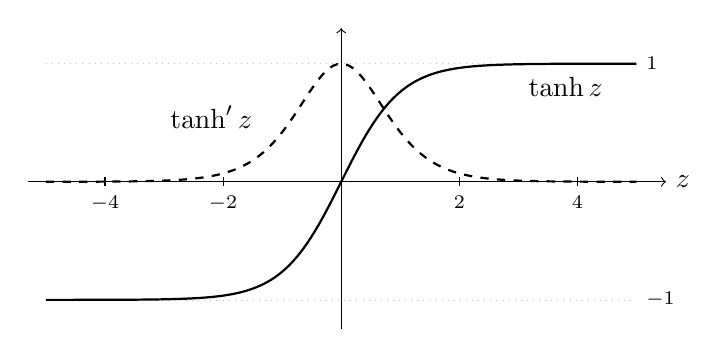
\begin{tikzpicture}[x=0.75cm,y=1.5cm]
  \axes{-5.3}{5.5}{-1.25}{1.3}
  \draw[guide] (-5,1) -- (5,1);
  \draw[guide] (-5,-1) -- (5,-1);
  \node[right] at (5,1) {\scriptsize $1$};
  \node[right] at (5,-1) {\scriptsize $-1$};
  \draw[fn, domain=-5:5] plot (\x, {tanh(\x)});
  \draw[dfn, domain=-5:5] plot (\x, {1-tanh(\x)*tanh(\x)});
  \node at (3.8,0.8) {$\tanh z$};
  \node at (-2.2,0.55) {$\tanh' z$};
\end{tikzpicture}
\caption{$\tanh$ (solid) and its derivative (dashed). Zero-centred, peak slope $1$.}
\end{figure}

\end{document}
